\chapter{实验评估}
\section{实验设置}
本次实验的实验环境为Windows 10 64位的系统,CPU为四核Intel Xeon 3.3Ghz CPU,24G内存。代码实现环境为Python3.5配合TensorfFow1.8.0版本。

TensorFlow是谷歌旗下的一款深度学习框架, 是一个使用数据流图进行数值计算的开放源代码软件库,利用TensorFlow框架可以轻松实现深度学习模型而不需要考虑算法的底层实现,并且TensorFlow提供多个优化器可供选择,其灵活的参数设置机制让使用者能够快速调整深度学习模型。因为其方便性与易用性,TensorFlow已经成为了机器学习工作者实现其模型的首选框架,这也是本文采用TensorFlow实现稳中算法的原因。

本文采用的数据集共12780个样例,其中5340个样例为不含空指针的正确代码,7440个样例为含空指针的缺陷代码。由于对于无缺陷代码的检测率四个工具检测准确率都较高,区分度较小,训练数据时限制了正确代码的数量,随机抽取了1000了个样例进行训练。去除掉一些节点数量异常大和数据过于稀疏的样例,总共有7638个样例进行训练,对于训练集数据,各个工具的检测结果分布如表\ref{tt}:

\begin{table}[ht]
	\centering
	\caption{训练集上工具检测结果}
	\label{tt}
	\begin{tabular*}{0.9\textwidth}{@{\extracolsep{\fill}}cccc}
		\toprule
		工具	&正确数量&错误数量&准确率	 \\
		\midrule
		FindBugs&5834&1488&76.68\%\\
		Infer&5102&2761&64.89\%\\
		Jlint&4964&2855&63.49\%\\
		Fortify&3917&3721&51.28\%\\
		\bottomrule
	\end{tabular*}
\end{table}

从上表可以看到即使是准确率最低的工具Fortify也达到了50\%以上的准确率,如果直接将这批训练集放入模型训练的话,因为正负样本数量分布不均的情况,很容易出现模型直接收敛到样本多数值的问题,造成最终的模型训练效果低下。为了解决样本分布不均的问题,本文试验了两种常用的方法,过采样和欠采样的方法。过采样方法随机重复采样数量较少的样本,从而达到正负样本数量均衡的效果,不过重复的采样容易导致过拟合的问题。欠采样的方法随机丢弃一些多数样本的数据,在训练模型时保持正负样本数据数量的一致。
%依然在浮动图环境中
\begin{figure}[h]
	%盒子一
	\parbox[h]{.5\textwidth}{\centering
		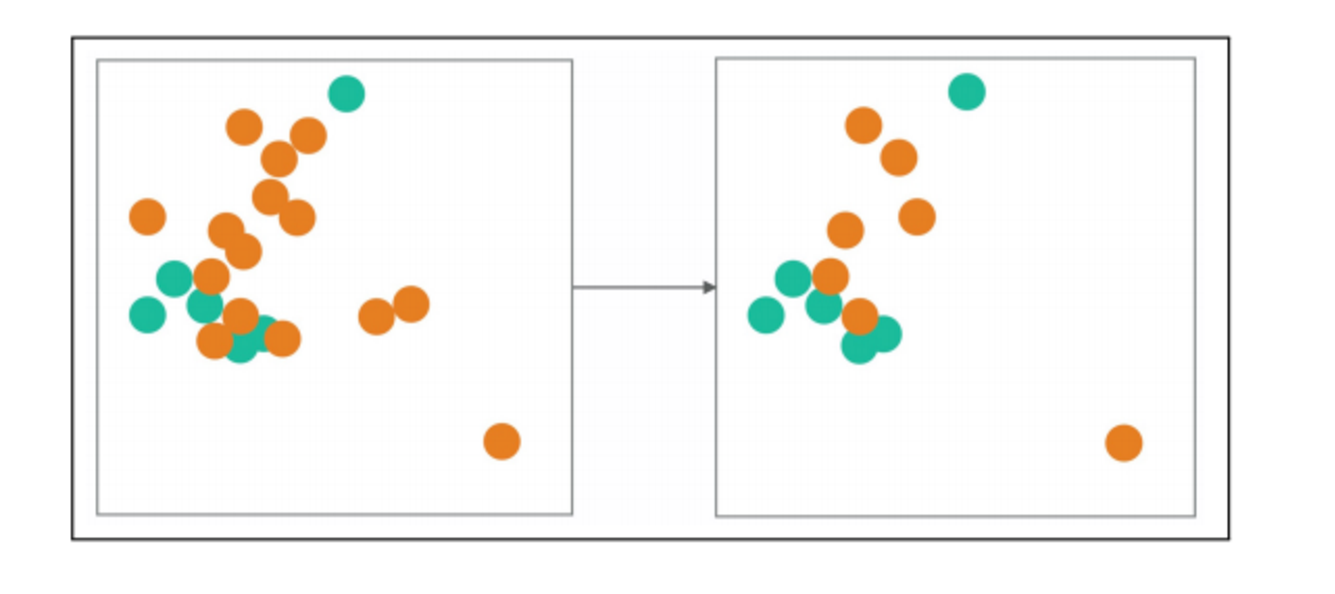
\includegraphics[width=0.45\textwidth]{figures/7.pdf}
		\caption{欠采样方法示例}}
	%盒子二
	\parbox[h]{.5\textwidth}{\centering
		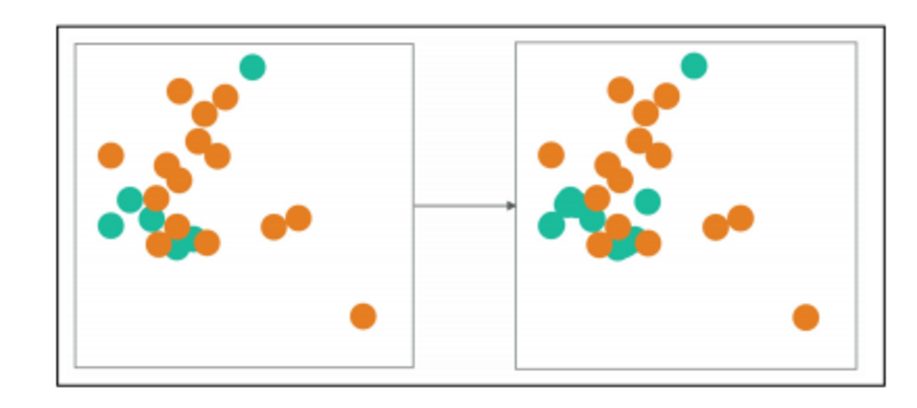
\includegraphics[width=0.45\textwidth]{figures/8.pdf}
		\caption{过采样方法示例}}
\end{figure}

经过对比,本文选择了欠采样的方法。例如针对FindBugs工具,训练时在5834个检测正确的样本中随机挑选出1488个,与1488个缺陷样本一起加入训练,保证了训练数据正负样本的数量均衡。随机欠采样的方法既不会影响数据的统计特征,同时可以使正负样本的边界更为清晰。本文的测试数据采用了不同于训练数据的1000个代码样例,同样的,为了保证样本正负样本数量的均衡,每次测试时,本文从1000个样本中随机抽取正负样本各50个进行测试,测试十次得到测试的平均正确率。

\section{训练设置}
本次模型训练采用了TensorFlow的AdamOptimizer,AdamOptimizer实现了Adam优化算法,比起随机梯度下降的方法,Adam算法收敛速度更加迅速,陷入局部最优解的概率更小。训练学习率初始设置为$10^{4}$,学习率随着训练的迭代步数增加而呈阶梯状下降,每迭代100次变为原来的0.98倍。损失函数采用了交叉熵的算法。对两个概率分布$p$和$q$,通过$q$来表示$q$的交叉熵为:
$$H(p,q) = -\sum_x p(x)\log q(x)$$

通过交叉熵函数可以比较两个概率分布的差异。交叉熵越小,表示两个概率分布差异越小,优化器可以根据交叉熵的值更新模型。

针对本文提出的模型,有两个参数可能影响模型的结果:图压缩后特征向量的维度大小$d$以及压缩算法的迭代次数$T$。接下来将分别探讨两者的影响。


对于特征向量$d$,可以看出,当$d$的维度增加,网络中的参数$W_1, W_2, W_3, W_4$的维度都会相应的增加,相当于网络的每一层的神经元都会增加,网络变得更加复杂,能够拟合的函数也就越复杂,于此同时模型的训练难度和时间消耗也会增加。网络如果过于负载也有可能导致模型过拟合的问题。

对于循环次数$T$,相类似的,随着循环次数的增加,网络的层数逐渐增加,网络更加复杂,拟合的函数越复杂,同时也可能会发生训练时间过长和过拟合的问题。

为了找到最佳的特征向量维度$d$以及迭代次数$T$,本文在迭代次数1到4下特征维度8到512维之间进行了实验,采用了最佳的组合:循环次数为3,特征向量维度为32维。
\begin{figure}[htbp]
	\begin{center}
		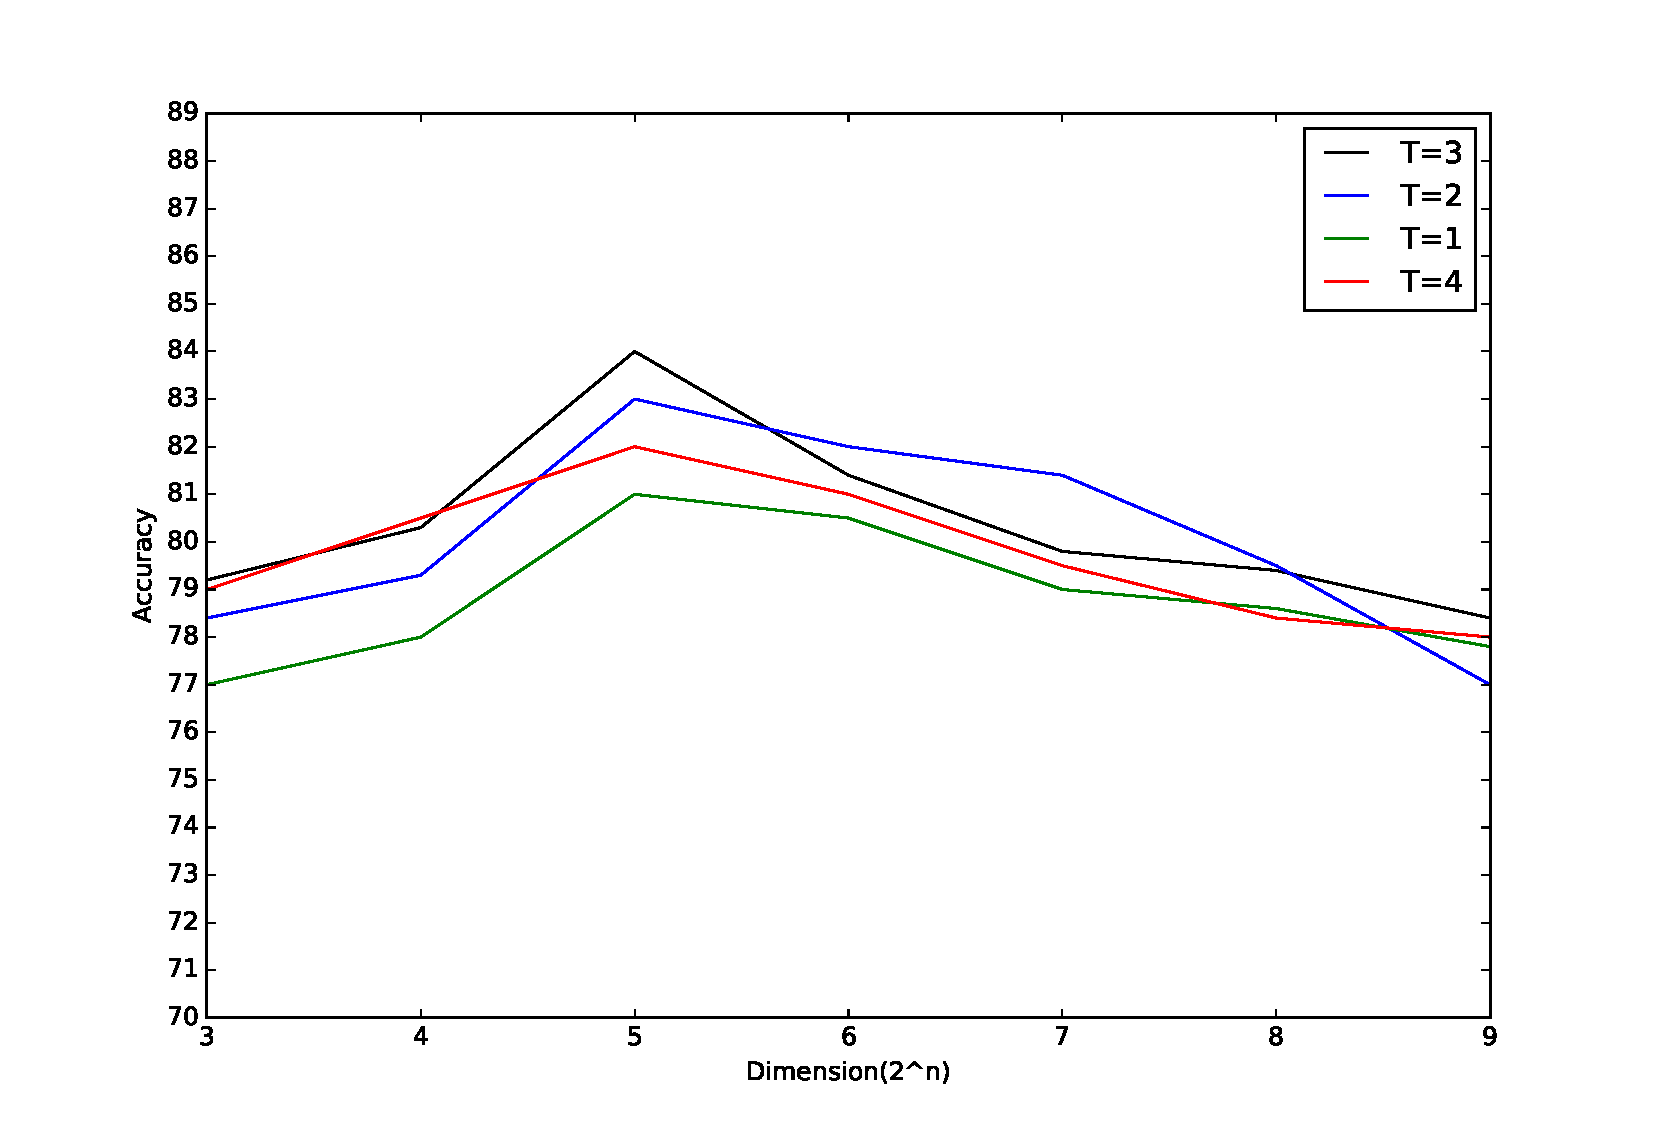
\includegraphics[width=0.95\textwidth]{figures//9.pdf}
		\caption{不同组合的准确率}
		\label{default}
	\end{center}
\end{figure}
\section{实验结果}
得到四个分类器后,可以综合分类器的结果和四个工具的检测结果进行空指针判定。为了增加工具检测含空指针和不含空指针数据之间的差异,本文对标签进行了预处理,当工具检测含空指针时,置为1;工具检测不含空指针时,置为0。这样得到四个工具的检测结果向量$R={r_1, r_2, r_3, r_4}$,模型得出的四个工具的置信度矩阵$W={w_1, w_2, w_3, w_4}$,这样测试样例是否含有空指针的置信度为$P = W^T*R = \sum_{i=1}^4 w_i*r_i$。可以设定一个阈值$p$, 当$P>=p$时判定该代码存在空指针缺陷。

当模型分类完全没有误差时,阈值$p$应该接近于0。然而在现实中模型完全没有误差是不可能的,因此$p$的值并不能单纯取0,为了得到$p$最佳的取值,本文选取了从-0.3到0.4,每隔0.05取一个阈值进行实验。实验从测试集中随机选取了100个样例,对这100个样例进行空指针检测以及模型检验,计算空指针检测准确率后得到表\ref{res}的结果:
\begin{figure}[htbp]
	\begin{center}
		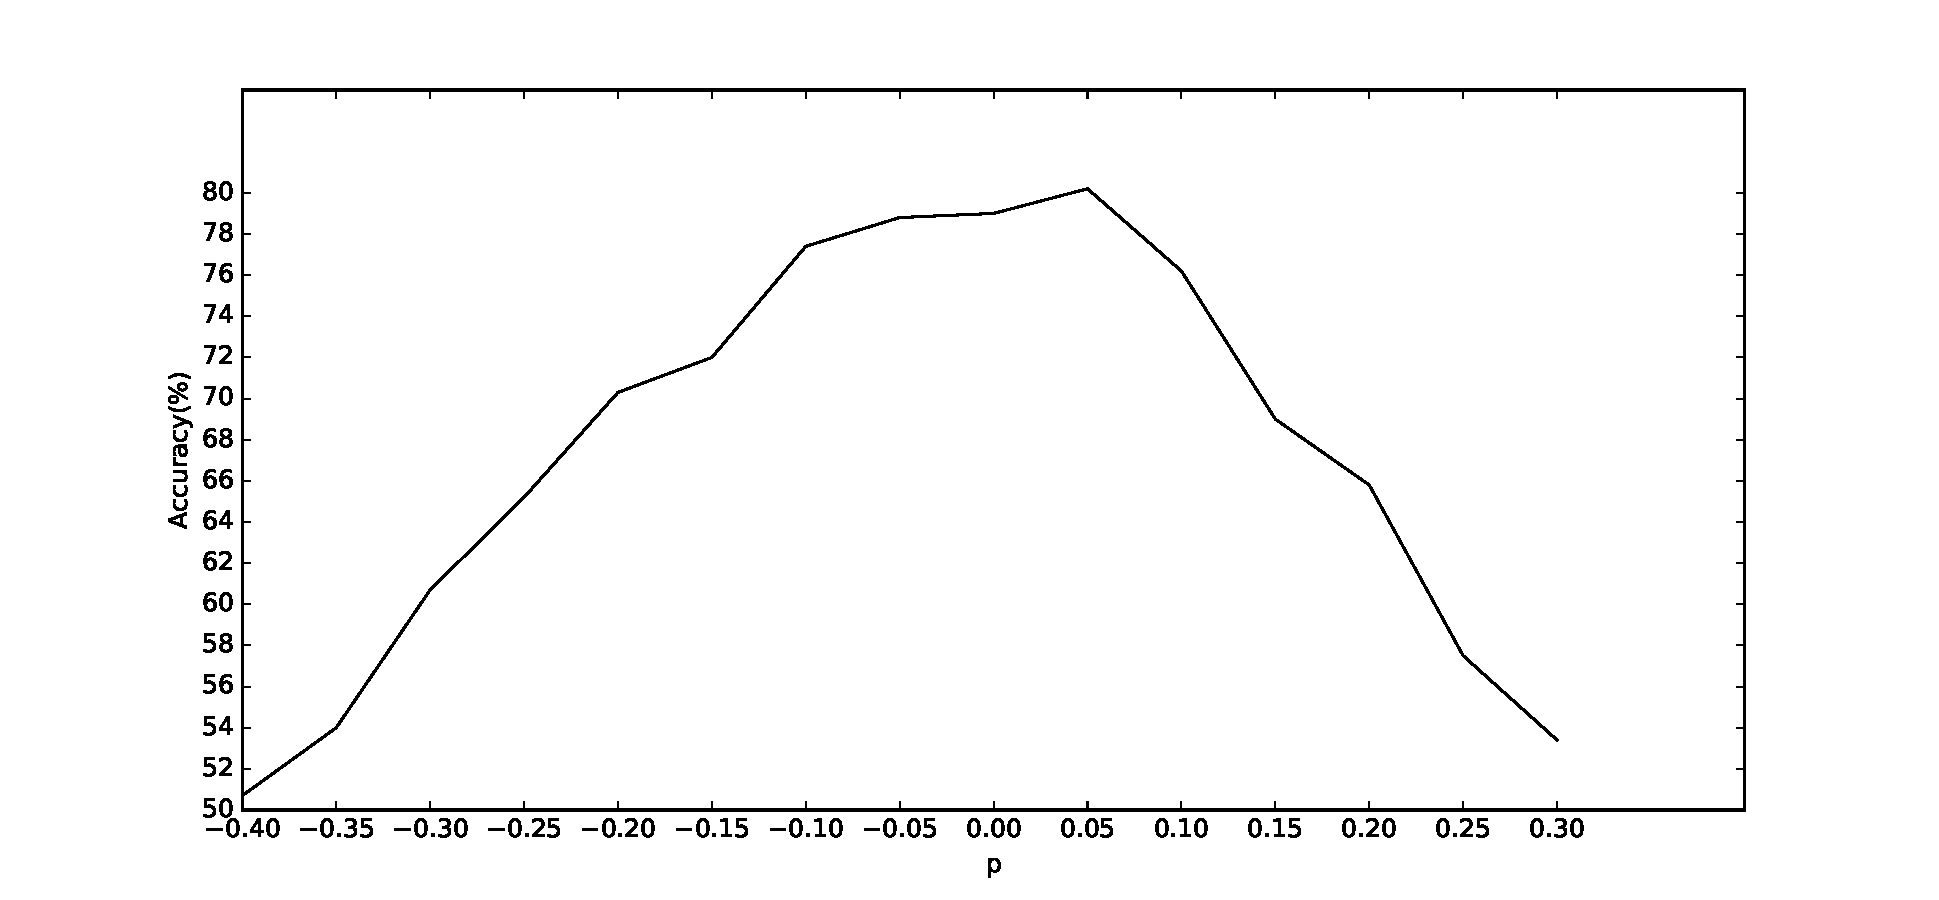
\includegraphics[width=0.95\textwidth]{figures//10.pdf}
		\caption{不同阈值下的空指针检测准确率}
		\label{res}
	\end{center}
\end{figure}
